\documentclass{article}
\usepackage[left=3cm,right=3cm,top=2cm,bottom=2cm]{geometry} % page
                                                             % settings
\usepackage{amsmath} % provides many mathematical environments & tools
\usepackage{amsfonts}
\usepackage[spanish]{babel}
\usepackage[doument]{ragged2e}

\usepackage{wasysym}

% Images
\usepackage{graphicx}
\usepackage{float}

% Code
\usepackage{listings}
\usepackage{xcolor}
\definecolor{gray}{rgb}{0.5,0.5,0.5}
\newcommand{\n}[1]{{\color{gray}#1}}
\lstset{numbers=left,numberstyle=\small\color{gray}}

\selectlanguage{spanish}
\usepackage[utf8]{inputenc}
\setlength{\parindent}{0mm}

\usepackage{pdfpages}

\begin{document}
\title{Aprendizaje Automático: Cuestionario 2, ejercicio 5}
\author{David Cabezas Berrido}
\maketitle

\section{Grafo del modelo:}

\begin{figure}[H]
  \centering
  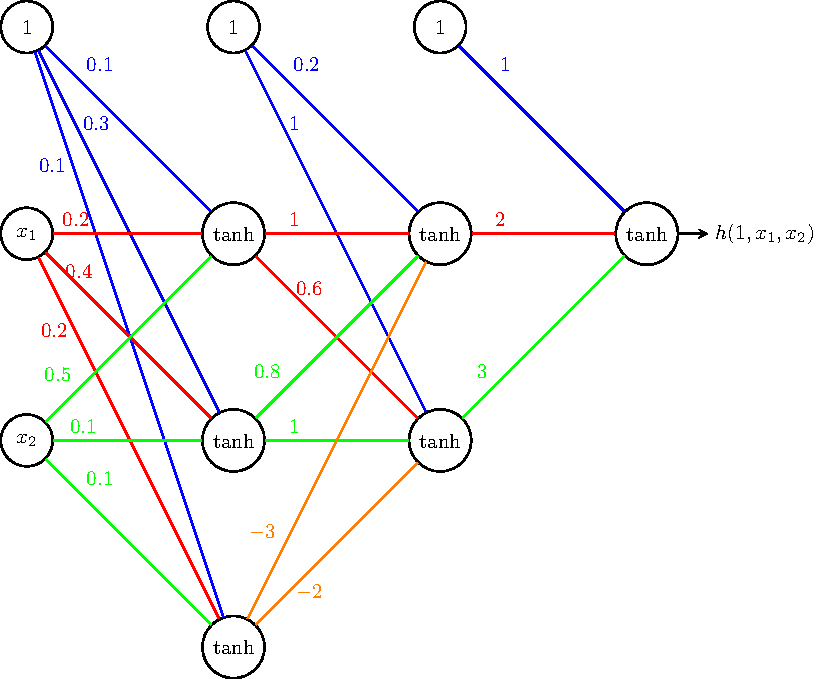
\includegraphics[width=180mm]{grafo5.pdf}
  \caption{Grafo de la Red Neuronal}
  \label{fig:graph-nn}
\end{figure}

\newpage
\section{Propagación hacia delante}

\[\textbf{x}^{(0)}=\begin{pmatrix}
    1 \\ 2 \\ 2 
  \end{pmatrix}\]

\[\textbf{s}^{(1)}=W_0^T\textbf{x}^{(0)}=\begin{pmatrix}
    1.5 \\ 1.3 \\ 0.7
  \end{pmatrix}\]

\[\textbf{x}^{(1)}=\begin{pmatrix}1 \\
    \tanh(\textbf{s}^{(1)})\end{pmatrix}=\begin{pmatrix} 1 \\ 0.90514825 \\
    0.86172316 \\ 0.60436778
  \end{pmatrix}\]

\[\textbf{s}^{(2)}=W_1^T\textbf{x}^{(1)}=\begin{pmatrix}
    -0.01857655 \\ 1.19607656
  \end{pmatrix}\]

\[\textbf{x}^{(2)}=\begin{pmatrix}1 \\
    \tanh(\textbf{s}^{(2)})\end{pmatrix}=\begin{pmatrix} 1 \\ -0.01857441 \\
   0.83245396
 \end{pmatrix}\]

\[\textbf{s}^{(3)}=W_3^T\textbf{x}^{(2)}=\begin{pmatrix}
    3.46021305
  \end{pmatrix}\]

\[\textbf{x}^{(3)}=\begin{pmatrix}1 \\
    \tanh(\textbf{s}^{(3)})\end{pmatrix}=\begin{pmatrix} 1 \\ 0.99802713
  \end{pmatrix}\]

La red precide $h(\textbf{x})=0.99802713$ y la etiqueta es $1$, así
que el error es $\textbf{e}=(h(\textbf{x};\textbf{w})-y)^2=(0.99802713-1)^2=3.8922\cdot 10^{-6}$.

\section{Propagación hacia atrás}

Sensibilidades:

\[\boldsymbol{\delta}^{(3)}=\frac{\partial\textbf{e}}{\partial\textbf{s}^{(3)}}=2(\textbf{x}^{(3)}-y)\tanh'(\textbf{s}^{(3)})=2(\textbf{x}^{(3)}-y)(1-\textbf{x}^{(3)}\astrosun\textbf{x}^{(3)})=-1.555351\cdot 10^{-5}\]

\[\boldsymbol{\delta}^{(2)}=\frac{\partial\textbf{e}}{\partial\textbf{s}^{(2)}}=\tanh'(\textbf{s}^{(2)})\astrosun[W^{(3)}\boldsymbol{\delta}^{(3)}]_1^2=\begin{pmatrix} -3.10962877\cdot 10^{-5} \\ -1.43257349\cdot 10^{-5} \end{pmatrix}\]

\[\boldsymbol{\delta}^{(1)}=\frac{\partial\textbf{e}}{\partial\textbf{s}^{(1)}}=\tanh'(\textbf{s}^{(1)})\astrosun[W^{(2)}\boldsymbol{\delta}^{(2)}]_1^3=\begin{pmatrix} -7.17255887\cdot 10^{-6} \\ -1.00920931\cdot 10^{-5} \\ 7.74003569\cdot 10^{-5}\end{pmatrix}\]

Derivadas respecto a los errores:

\[\frac{\partial\textbf{e}}{\partial W^{(1)}}=\textbf{x}^{(0)}[\boldsymbol{\delta}^{(1)}]^T=\begin{pmatrix} -7.17255887\cdot 10^{-6} & -1.00920931\cdot 10^{-5} & 7.74003569\cdot 10^{-5} \\
    -1.43451177\cdot 10^{-5} & -2.01841863\cdot 10^{-5} & 1.54800714\cdot 10^{-4} \\ -1.43451177\cdot 10^{-5} & -2.01841863\cdot 10^{-5} & 1.54800714\cdot 10^{-4} \end{pmatrix}\]

\[\frac{\partial\textbf{e}}{\partial W^{(2)}}=\textbf{x}^{(1)}[\boldsymbol{\delta}^{(2)}]^T=\begin{pmatrix} -3.10962877\cdot 10^{-5} & -1.43257349\cdot 10^{-5} \\
       -2.81467505\cdot 10^{-5} & -1.29669139\cdot 10^{-5} \\
       -2.67963913\cdot 10^{-5} & -1.23448176\cdot 10^{-5} \\
       -1.87935943\cdot 10^{-5} & -8.65801257\cdot 10^{-6}
     \end{pmatrix}\]

\[\frac{\partial\textbf{e}}{\partial W^{(3)}}=\textbf{x}^{(2)}[\boldsymbol{\delta}^{(3)}]^T=\begin{pmatrix} -1.55535099\cdot 10^{-5} \\
       2.88897328\cdot 10^{-7} \\
       -1.29475809\cdot 10^{-5} 
  \end{pmatrix}\]

\end{document}